\begin{frame}
    \begin{center}
        \small
        Волгоградский Государственный Технический Университет \\
        Факультет электроники и вычислительной техники \\
        Кафедра САПРиПК \\
        \vspace{1.5cm}
        \normalsize
        \textbf{Метод кластеризации предпочтений жителей города по
        перемещению.}\\
        \vspace{1.0cm}
        \raggedleft\small
        \textbf{Исполнитель:}\\Чечеткин~И.~А.\\
        \textbf{Руководитель:}\\Щербаков~М.~В.\\
        \vspace{1.5cm}
        \vspace{\fill}
        \centeringВолгоград \the\year
    \end{center}
\end{frame}

\begin{frame}
    \frametitle{Формулировка проблемы}
    \textbf{Актуальность.} В настоящее время формирование маршрутов в городской
    среде осуществляется на основе положений, заложенных в городской план
    развития. Обычно, эта информация достаточно устаревшая и не учитывает
    предпочтения жителей. На основе данных о предпочтениях жителей требуется
    разработать эффективный метод кластеризации предпочтений жителей города
    по перемещению.\\
    \textbf{Объект исследования} -- предпочтения жителей города, выраженные
      в географических координатах.\\
    \textbf{Предмет исследования} -- методы кластеризации предпочтений жителей.
\end{frame}

\begin{frame} % Слайд 3
    \frametitle{Цели и задачи}
    \textbf{Цель работы} -- разработка метода кластеризации предпочтений
    жителей для минимизации дискомфорта перемещения в городе.\\
    \textbf{Теоретические задачи:}
    \begin{itemize}
        \item разработка алгоритма кластеризации;
        \item разработка метода учета географических особенностей местности;
        \item разработка критериев для оценки качества кластеризации.
    \end{itemize}
    \textbf{Практические задачи:}
    \begin{itemize}
        \item генерация исходных данных;
        \item реализация разработанных алгоритмов и методов;
        \item построение полученных результатов на карте;
        \item оценка качества кластеризации.
    \end{itemize}
\end{frame}

\begin{frame}
    \frametitle{Понятийный аппарат}
    \footnotesize
    \begin{itemize}\itemsep-5pt
        \item \textbf{Предпочтение} -- пара узлов с определенными координатами
            и идентификатором пользователя.
        \item \textbf{Node (узел)} -- точка с указанными координатами и тегами.
        \item \textbf{Tag (тег)} -- пары <<ключ -- значение>>.
        \item \textbf{Дискомфорт} -- совокупный параметр, определяющий время
            перемещения из начального узла в конечный.
        \item \textbf{Центроид} -- центр тяжести фигуры (геометрический центр).
        \item \textbf{Метрика} -- функция, определяющая расстояние в
            метрическом пространстве.
        \item \textbf{Framework (фреймворк)} -- программное обеспечение, облегчающее разработку и
            объединение разных компонентов большого программного проекта.
        \item \textbf{OpenStreetMap (OSM)} -- некоммерческий веб-картографический проект по созданию
            сообществом подробной свободной и бесплатной географической карты мира.
        \item \textbf{Project OSRM} -- фреймворк для вычисления кратчайших путей в графе дорог.
            Разработан для использования с картографическим сервисом OSM.
    \end{itemize}
\end{frame}

\begin{frame}
    \frametitle{Список литературы}
    \begin{enumerate}
        \scriptsize
        \item[1] Воронцов, К. В. Машинное обучение.~--- Режим доступа:\\
            \url{http://www.machinelearning.ru/}\\
        \item[2] Mean Shift Clustering. --- Available at:\\
            {\tiny\url{http://homepages.inf.ed.ac.uk/rbf/CVonline/LOCAL_COPIES/TUZEL1/MeanShift.pdf}}
        \item[3] Comaniciu, D. Mean Shift: A Robust Approach Toward Feature Space Analysis.~/
            D. Comaniciu, P. Meer.~--- Available at:\\
            \url{https://courses.csail.mit.edu/6.869/handouts/PAMIMeanshift.pdf}
        \item[4] Allard, D. Clustering geostatical data.~/
            D. Allard, G. Guillot.~--- Available at:\\
            \url{http://people.compute.dtu.dk/gigu/article_capetown.pdf}\\
        \item[5] Scikit learn: clustering.~--- Available at:\\
            \url{http://scikit-learn.org/stable/modules/clustering.html}
    \end{enumerate}
\end{frame}

\begin{frame}
    \frametitle{Исходная выборка}
    \begin{figure}
        \center
        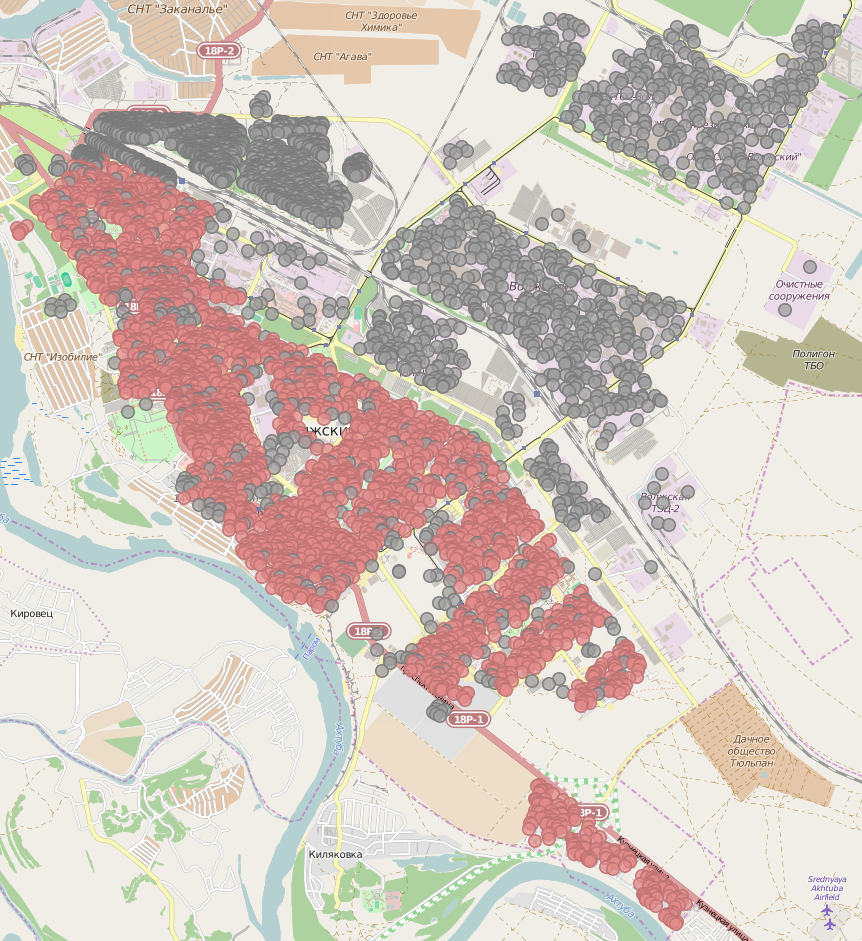
\includegraphics[width=.7\textwidth]{map}
    \end{figure}
\end{frame}

\begin{frame}
    \frametitle{Используемый алгоритм}
    Псевдокод алгоритма Mean Shift:\\
    \begin{enumerate}\itemsep -.5ex
        \item Генерирование начального распределения центроидов
        \item \textbf{ПОВТОРЯТЬ}
        \item Определение соседних точек к центроидам
        \item Определение среднего веса соседних точек к центроидам
        \item Рассчет нового положения центроидов
        \item Сдвиг центроидов
        \item \textbf{ПОКА} разница между рассчитанным положением и текущим не будет равна 0
        \item \textbf{ВЫВОД} центроиды
    \end{enumerate}
\end{frame}

\begin{frame}
    \frametitle{До оптимизации}
    \begin{figure}
        \center
        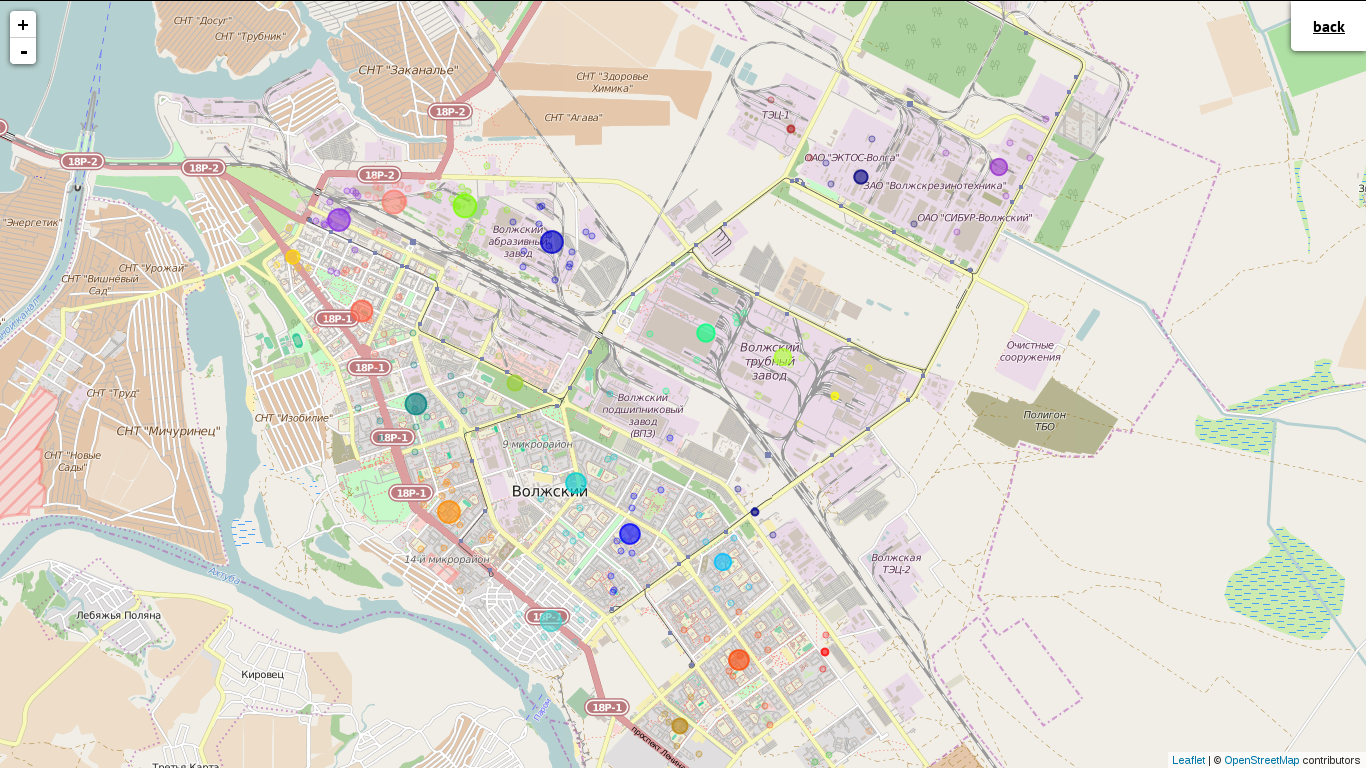
\includegraphics[width=\textwidth]{eu}
    \end{figure}
\end{frame}

\begin{frame}
    \frametitle{После оптимизации}
    \begin{figure}
        \center
        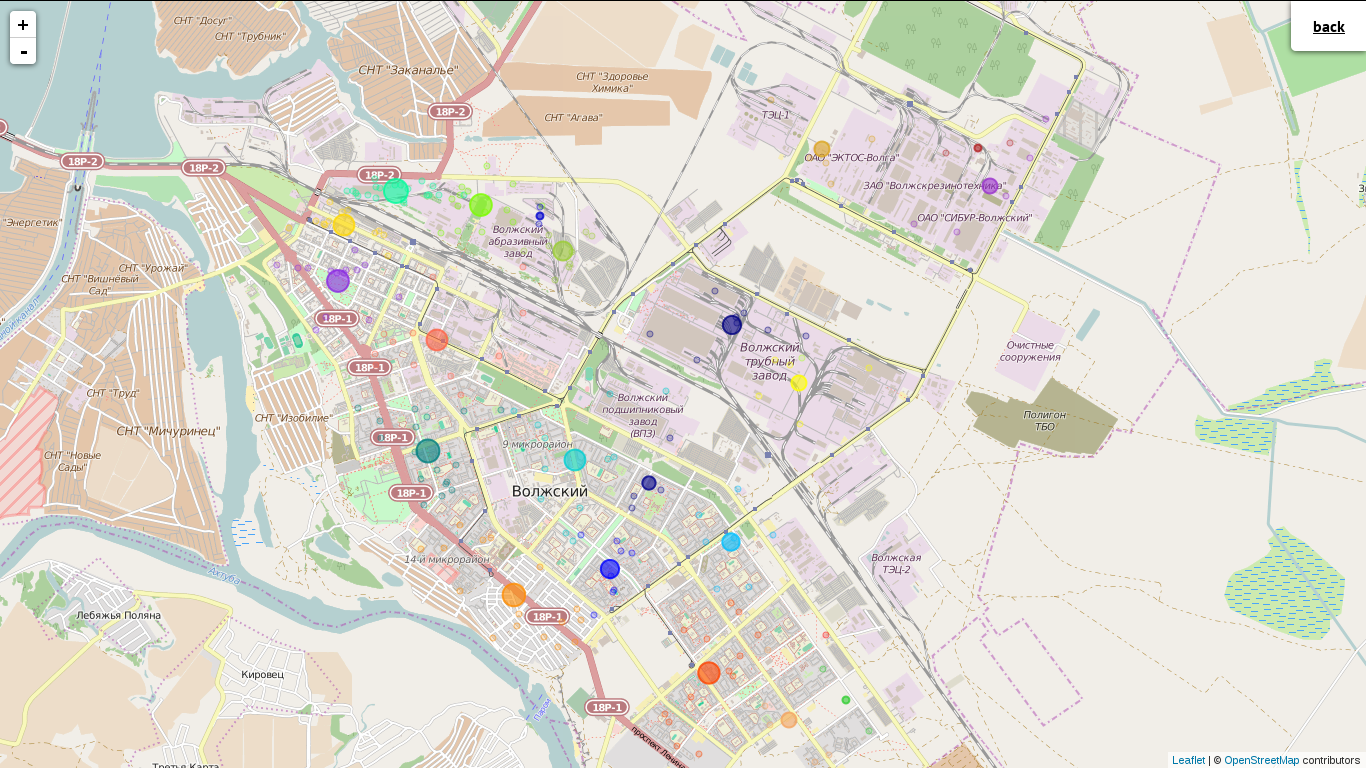
\includegraphics[width=\textwidth]{rou}
    \end{figure}
    \small\emph{Реализованный алгоритм:} \url{https://github.com/vstu-cad-stuff/clustering}
\end{frame}

\begin{frame}
    \frametitle{Прототип}
    \begin{figure}
        \center
        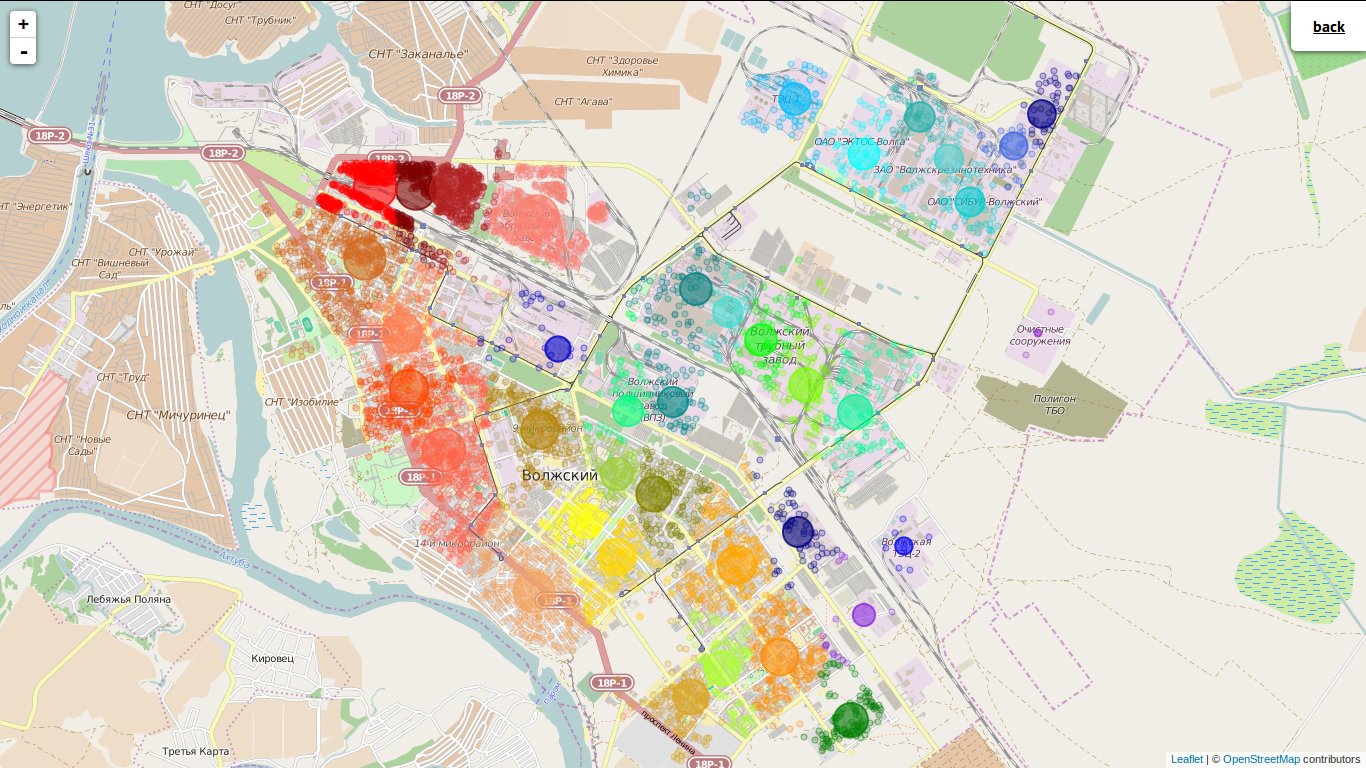
\includegraphics[width=\textwidth]{proto}
    \end{figure}
    \small\emph{Ссылка на приложение:} \url{http://vstu-cad-stuff.github.io/clustering/}
\end{frame}
